\documentclass[
  captions=tableheading,
  bibliography=totoc, 
  titepage=firstiscover,
]{scrartcl}

\usepackage{blindtext} %neuer input

\usepackage{longtable} % Tabellen über mehrere Seiten

\usepackage[utf8]{inputenc} %neuer input

\usepackage{scrhack}

\usepackage[aux]{rerunfilecheck} %Warnung falls nochmal kompiliert werden muss

\usepackage{fontspec} %Fonteinstellungen

\recalctypearea{}

\usepackage[main=ngerman]{babel} %deutsche Spracheinstellung

\usepackage{ragged2e} %neuer input

\usepackage{amsmath, nccmath}

\usepackage{amssymb} %viele mathe Symbole

\usepackage{mathtools} %Erweiterungen für amsmath


\DeclarePairedDelimiter{\abs}{\lvert}{\rvert}
\DeclarePairedDelimiter{\norm}{\lVert}{\rVert}

\DeclarePairedDelimiter{\bra}{\langle}{\rvert}
\DeclarePairedDelimiter{\ket}{\lvert}{\rangle}

\DeclarePairedDelimiterX{\braket}[2]{\langle}{\rangle}{
#1 \delimsize| #2
}

\NewDocumentCommand \dif {m}
{
\mathinner{\symup{d} #1}
}


\usepackage[
  math-style=ISO,
  bold-style=ISO,
  sans-style=italic,
  nabla=upright,
  partial=upright,
  warnings-off={
    mathtools-colon,
    mathtools-overbracket,
  },
]{unicode-math}

\setmathfont{Latin Modern Math}
\setmathfont{XITS Math}[range={scr, bfscr}]
\setmathfont{XITS Math}[range={cal, bfcal}, StylisticSet=1]


\usepackage[
  locale=DE,
  separate-uncertainty=true,
  per-mode=reciprocal,
  output-decimal-marker={,},
]{siunitx}

\usepackage[autostyle]{csquotes} %richtige Anführungszeichen

\usepackage{xfrac}

\usepackage{float}

\floatplacement{figure}{htbp}

\floatplacement{table}{htbp}

\usepackage[ %floats innerhalb einer section halten
  section,   %floats innerhalb er section halten
  below,     %unterhalb der Section aber auf der selben Seite ist ok
]{placeins}

\usepackage[
  labelfont=bf,
  font=small,
  width=0.9\textwidth,
]{caption}

\usepackage{subcaption} %subfigure, subtable, subref

\usepackage{graphicx}

\usepackage{grffile}

\usepackage{booktabs}

\usepackage{microtype} %Verbesserungen am Schriftbild

\usepackage[
backend=biber,
]{biblatex}

\addbibresource{../lit.bib}

\usepackage[ %Hyperlinks im Dokument
  german,
  unicode,
  pdfusetitle,
  pdfcreator={},
  pdfproducer={},
]{hyperref}

\usepackage{bookmark}

\usepackage[shortcuts]{extdash}

%\usepackage{warpcol}


\begin{document}
    \title{Physik IV Übungsblatt 1}
    \author{  
    Tobias Rücker\\
    \texorpdfstring{\href{mailto:tobias.ruecker@tu-dortmund.de}{tobias.ruecker@tu-dortmund.de}
    \and}{,} 
    Paul Störbrock\\
    \texorpdfstring{\href{mailto:paul.stoerbrock@tu-dortmund.de}{paul.stoerbrock@tu-dortmund.de}}{}
    }
\maketitle
\center{\Large Abgabegruppe: \textbf{4 H}}
\thispagestyle{empty}

\newpage
\tableofcontents
\thispagestyle{empty}
\newpage

\setcounter{page}{1}


\section{Aufagabe 1}

\subsection{a)}

\begin{figure}[H]
    \centering
    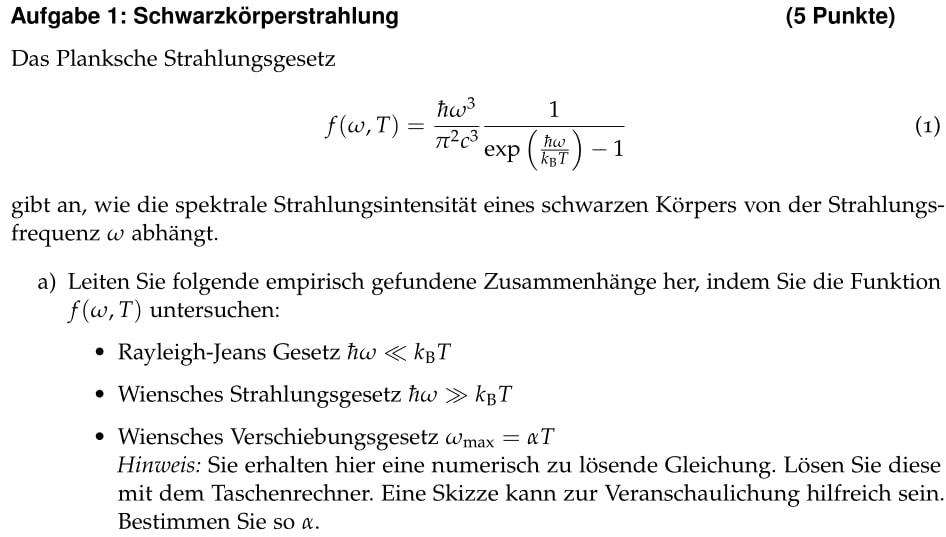
\includegraphics[width=0.75\textwidth]{images/Aufgabe_1a.jpg}
    \label{fig:1}
\end{figure}


Herleitung des Rayleigh-Jeans Gesetz aus dem Plank'schen Strahlungsgesetz:

\begin{align*}
    f(\omega , T)&= \frac{\hbar \omega ^3}{\pi ^2 c^3} \frac{1}{\text{exp}\left(\frac{\hbar \omega}{k_{\text{B}} T} \right)-1}
    \intertext{
        \flushleft{Da\;}\justifying $\hbar \omega \ll k_{\text{B}}T$ ist, wird der Expontialteil ebenso sehr klein,
        wodurch dieser näherungsweise durch sein erstes Taylorpolynom $T(e^x,0)=1+x$ dargestellt werden kann.
        Daraus folgt dann:
    }
    f(\omega , T) &\approx \frac{\hbar \omega ^3}{\pi ^2 c^3} \frac{1}{1+\frac{\hbar \omega}{k_{\text{B}} T} -1}\\
    &\Leftrightarrow  \frac{\omega ^2 k_{\text{B}}}{\pi ^2 c^3}\; T
    \intertext{
        Durch Ergänzung von $d \omega$ ergibt sich das Rayleigh-Jeans Gesetz
    }
    f(\omega, T) \, d \omega &= \frac{\omega ^2 k_{\text{B}}}{\pi ^2 c^3}\; T \, d \omega
\end{align*}

Herleitung des Wienschen Strahlungsgesetz Gesetz aus dem Plank'schen Strahlungsgesetz:

\begin{align*}
    \intertext{
        Für den Fall  $\hbar \omega \gg k_{\text{B}} T $ ist die Exponential viel größer als 1,
        so dass die 1 im Nenner vernachlässigt werden kann.
        Mit
    }
    c_1 = \frac{\hbar}{\pi ^2 c^3} \;\text{und} \; c_2 = \hbar
    \intertext{
        ergibt sich das Wiensche Strahlungsgesetz:
    } 
    f(\omega, T) = c_1 \omega ^3 \exp \left(\--\frac{c_2 \omega}{k_B T} \right)
\end{align*}

Herleitung des Wienschen Verschiebungsgesetz aus dem Plank'schen Strahlungsgesetz:

Bedingung: $d_{\omega} f(\omega,T) = 0 $

\begin{align*}
    d_{\omega} f(\omega, T) &= \frac{\hbar }{\pi ^2 c^3} \frac{d}{d\omega} \frac{\omega^3}{\text{exp}\left(\frac{\hbar \omega}{k_{\text{B}} T} \right)-1}
    \intertext{
       Setze  
    }
    C &= \frac{\hbar }{\pi ^2 c^3}\\
    C'&= \frac{\hbar}{k_{\text{B}}T}\\
    \Leftrightarrow C \frac{d}{d \omega} \frac{\omega ^3}{\exp (C' \omega)-1} &= 0\\
    \Leftrightarrow C \frac{3\omega ^2 (\exp(C' \omega)-1)-\omega ^3 C' \exp(C' \omega)}{(\exp(C' \omega)-1)^2} &= 0\\
    \intertext{
        Zähler muss null werden
    }
    C (3 \omega ^2(\exp(C' \omega)-1)- \omega ^3 C' \exp(C' \omega))&=0\\
    \Leftrightarrow C \omega ^2 (3 (\exp(C' \omega)-1)- \omega  C' \exp(C' \omega))&=0\\
    \Leftrightarrow 3 (\exp(C' \omega)-1)- \omega  C' \exp(C' \omega)&=0\\
    \Leftrightarrow -3&= (C' \omega -3) \exp(C' \omega)
\end{align*}
\begin{figure}[H]
    \centering
    \caption{numerische Lösung der Gleichung mit WolframAlpha}
    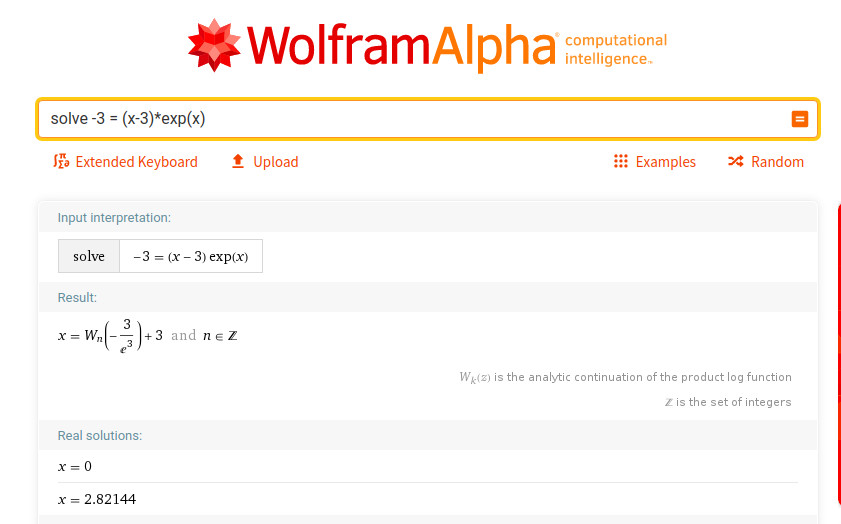
\includegraphics[width=0.75\textwidth]{images/wolfram_calc.jpg}
    \label{fig:2}
\end{figure}

\begin{align*}
    C' \omega &= 2.282144\\
    \omega &= \frac{1}{C'} 2.282144\\
     &= \frac{k_{\text{B}}}{\hbar}\cdot 2.282144\cdot T\\
    \omega &= \SI{3,6938e11}{\hertz\kelvin\tothe{-1}}\cdot T\\
    \alpha &= \SI{3,6938e11}{\hertz\kelvin\tothe{-1}}
\end{align*}

\subsection{b)}

\begin{figure}[H]
    \centering
    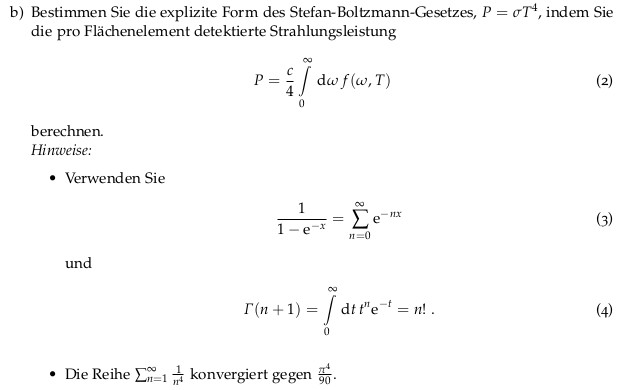
\includegraphics[width=0.75\textwidth]{images/Aufgabe_1b.jpg}
    \label{fig:3}
\end{figure}

\begin{align}
    P &= \frac{c}{4} \int_0^{\infty} \, d \omega \frac{\hbar \omega ^3}{\pi ^2c^3} \frac{1}{\exp\left(\frac{\hbar \omega}{k_{\text{B}}T}\right)-1}\\
    &= \--\frac{\hbar}{4 \pi ^2 c^2} \int_0^ {\infty} \, d \omega \frac{\omega ^3}{1-\exp \left(\-- \left(\--\frac{\hbar \omega}{k_{\text{B}}T} \right)\right)}\\
    &= \-- \frac{\hbar}{4\pi ^2 c^2} \int_0^ {\infty} \, d \omega \omega ^3 \sum_{n=0}^{\infty} \exp\left(\--\left(\--n\frac{\hbar \omega}{k_{\text{B}}T}\right)\right)\\
    \intertext{
        Substitution
    }
    u &= \--\frac{n \hbar \omega}{k_{\text{B}}T}\\
    \omega &= \--\frac{u k_{\text{B}}T}{\hbar n}\\
    \frac{du}{d \omega}&= \--\frac{n \hbar}{k_{\text{B}}T}\\
    d \omega &= \--\frac{k_{\text{B}}T}{n \hbar} \,d u\\
    P&= \frac{\hbar k_{\text{B}}^4 T^4}{4 \pi ^2 c^2 \hbar ^4} \sum_{n=0}^ {\infty} \frac{1}{n^4}\int_0^{\infty} \, du u^3 e^ {-u}\\
    &= \frac{ k_{\text{B}}^4 T^4}{4 \pi ^2 c^2 \hbar ^3} \sum_{n=0}^ {\infty} \frac{1}{n^4} 3!\\
    &= \frac{3}{2 \pi ^2}\frac{ k_{\text{B}}^4 T^4}{ c^2 \hbar ^3} \frac{\pi ^4}{90}\\
    &= \frac{\pi ^2}{60} \frac{ k_{\text{B}}^4}{ c^2 \hbar ^3} T^4 \\
    &= \sigma T^4
\end{align}

\subsection{c)}

Bei der Berechnung des Integrals über das Rayleigh-Jones Gesetz kommt es zur sogenannten Ultraviolett-Katastrophe:
\begin{align*}
    \int_0^{\infty} I(\omega)\, d \omega=\int_0^{\infty} \frac{\omega ^2}{\pi ^2 c^3} k_{\text{B}} T \, d \omega = \infty .
\end{align*}
Das Integral existiert auf dem Intervall von $\omega \in [0, \infty) $ nicht und die Strahlungleistung wird unendlich.
Bei hohen Frequenzen wäre  zu erwarten, dass die Strahlungsintensität entsprechend der Boltzmann Verteilung geringer wird

\section{Aufgabe 2}

\subsection{a)}

\subsection{b)}

\subsection{c)}

\section{Aufgabe 3}

\subsection{a)}

\begin{figure}[H]
    \centering
    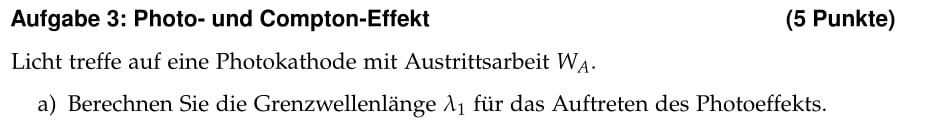
\includegraphics[width=0.75\textwidth]{images/Aufgabe_3a.jpg}
    \label{fig:8}
\end{figure}

    \flushleft{Damit\;}\justifying das Elektron der Kathode enkommen kann, muss das Photon Energie gleich der Austrittsarbeit ($W_A$) aufbringen. 
    Daraus folgt $\hbar \omega = W_A$.
    Wird nun für $\hbar$ und $\omega$

    \begin{align}
        \hbar &= \frac{h}{2\pi} \qquad \qquad \omega = \frac{c}{\lambda_1}\cdot 2\pi
                \intertext{eingesetzt, ergibt sich:
        }
        W_A &=\hbar \frac{c}{\lambda_1} 2 \pi \qquad \Leftrightarrow \qquad \lambda_1 = \frac{h c}{W_A}
    \end{align}

\subsection{b)}

\begin{figure}[H]
    \centering
    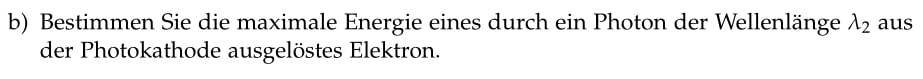
\includegraphics[width=0.75\textwidth]{images/Aufgabe_3b.jpg}
    \label{fig:9}
\end{figure}

    \flushleft{Die\;}\justifying maximale kinetische Energie ($E_{kin}$), die ein Elektron von einem Photon gewinnen kann, wird von der Austrittsarbeit beschränkt. 
    Daraus folgt:

    \begin{align}
        &E_{kin} = \hbar \omega_2 - W_A\\
        &E_{kin} = \frac{\hbar c}{\lambda_2} 2\pi - \frac{\hbar c}{\lambda_A} 2\pi = 
        \frac{h c}{\lambda_2} - \frac{h c}{\lambda_A} = h c \left ( \frac{1}{\lambda_2} - \frac{1}{\lambda_A} \right )
    \end{align}

\subsection{c)}

\begin{figure}[H]
    \centering
    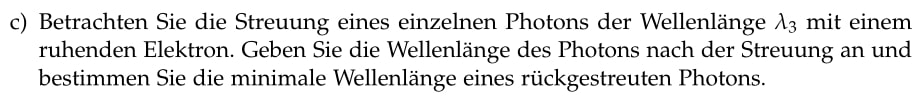
\includegraphics[width=0.75\textwidth]{images/Aufgabe_3c.jpg}
    \label{fig:10}
\end{figure}

    \flushleft{Mithilfe\;}\justifying von Energie- und Impulserhaltung lässt sich die Wellenlängendifferenz anhand des Steuungswinkels bestimmen.
    Energieerhaltung diktiert, dass die kinetische Energie des Photons ($h \omega$) plus der potentiellen Energie des Elektrons ($m_0 c^2$)
    gleich der Energie nach der Steuung sein muss. 
    Also folgt aus der

    \begin{align}
        &\text{Energieerhaltung}\;                          h\omega + m_0 \cdot c^2 = h\omega' + m \cdot c^2,\\
        &\text{der Impulserhaltung in x-Richtung}\;         \frac{h}{\lambda} = \frac{h}{\lambda'} \cdot cos(\phi) + m \cdot v \cdot cos(\theta)\\
        &\text{und der Impulserhaltung in y-Richtung}\;     0 = \frac{h}{\lambda'} \cdot sin(\phi) - m \cdot v \cdot sin(\theta)\\
        \intertext{die Wellenlängendifferenz
        }
        &\Delta\lambda = \lambda_3' - \lambda_3 = \frac{h}{m_0 c} \cdot (1-cos(\phi)). \label{eq:deltaL}\\
        \intertext{Die Wellenlänge wird minimal bei maximaler Frequenz, welche bei Rückstreuung auftritt. Werden
        }
        &\frac{h}{m_0 c} = \lambda_c = const \qquad \text{und} \qquad \phi = \pi 
        \intertext{in \eqref{eq:deltaL} eingesetzt, folgt die minimale Wellenlänge:
        }
        &\Rightarrow \lambda_3' = 2 \cdot \lambda_c + \lambda_3
    \end{align}

\subsection{d)}

\begin{figure}[H]
    \centering
    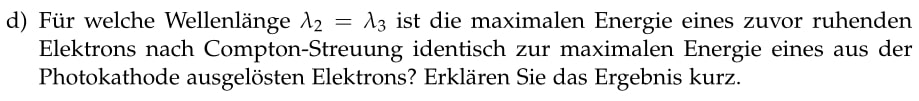
\includegraphics[width=0.75\textwidth]{images/Aufgabe_3d.jpg}
    \label{fig:11}
\end{figure}

\end{document}